\documentclass[11pt]{article}

% Mandatory Packages
\usepackage{amsmath}
\usepackage{amssymb}
\usepackage{amsthm}
\usepackage{geometry}
\usepackage{tikz}
\usetikzlibrary{arrows.meta, positioning, shapes, decorations.pathreplacing}
\usepackage{mathrsfs}
\usepackage{mathtools}

% Page Geometry
\geometry{letterpaper, margin=1in}

% Theorem Environments
\newtheorem{theorem}{Theorem}[section]
\newtheorem{lemma}[theorem]{Lemma}
\newtheorem{proposition}[theorem]{Proposition}
\newtheorem{corollary}[theorem]{Corollary}
\theoremstyle{definition}
\newtheorem{definition}{Definition}[section]
\newtheorem{axiom}{Axiom}[section]
\newtheorem{example}{Example}[section]
\theoremstyle{remark}
\newtheorem{remark}{Remark}[section]

% Title Information
\title{Homework 3: Hypergeometric and Poisson Distributions}
\author{Tashfeen Omran}
\date{September 2026}

\begin{document}

\maketitle
\tableofcontents
\newpage

\section{Part 1: Comprehensive Introduction, Context, and Prerequisites}

\subsection{Core Concepts \& Axioms}
In the rigorous study of probability theory, we operate within a probability space defined by the triplet $(\Omega, \mathcal{F}, \mathbb{P})$, where $\Omega$ is the sample space, $\mathcal{F}$ is a $\sigma$-algebra of events, and $\mathbb{P}$ is a probability measure. This chapter introduces two fundamental discrete probability distributions that model distinct physical phenomena: the \textbf{Hypergeometric Distribution} and the \textbf{Poisson Distribution}.

\begin{definition}[Hypergeometric Distribution]
Let a population of size $N$ be partitioned into two mutually exclusive sets: $r$ elements possessing a specific attribute (successes) and $N-r$ elements lacking it (failures). If a sample of size $n$ is drawn \textit{without replacement}, the random variable $Y$ representing the number of successes in the sample follows a Hypergeometric distribution. The probability mass function (PMF) is given by:
\[ P(Y = y) = \frac{\binom{r}{y}\binom{N-r}{n-y}}{\binom{N}{n}} \]
where $\max(0, n - (N-r)) \le y \le \min(n, r)$.
\end{definition}

\begin{definition}[Poisson Distribution]
A random variable $Y$ is said to have a Poisson distribution with rate parameter $\lambda > 0$ if it models the number of events occurring in a fixed interval of time or space, assuming these events occur with a known constant mean rate and independently of the time since the last event. The PMF is:
\[ P(Y = y) = \frac{\lambda^y e^{-\lambda}}{y!}, \quad y \in \{0, 1, 2, \dots\} \]
\end{definition}

\subsection{Intuition and Set-Theoretic/Logical Foundations}
From a set-theoretic perspective, the Hypergeometric distribution relies on the discrete counting measure. The sample space $\Omega$ consists of all $\binom{N}{n}$ possible subsets of size $n$. Because the draws are without replacement, the probability of selecting a success changes dynamically; the events are strictly \textit{dependent}. We partition the target subset into two intersections: one with the set of successes and one with the set of failures.

Conversely, the Poisson distribution can be viewed through the lens of measure theory as a Poisson Random Measure. It represents the limit of a Binomial distribution as the number of trials $n \to \infty$ and the probability of success $p \to 0$, such that $np = \lambda$ remains constant. It formalizes the concept of "rare events" occurring over a continuous continuum (like time $\mathbb{R}^+$).

\subsection{Historical Context and Motivation}
The Hypergeometric distribution was formalized during the development of quality control and acceptance sampling in the early 20th century. Industrial manufacturers needed a rigorous way to determine the probability of finding defective items in a finite batch without testing every single item (which is often destructive and costly). 

The Poisson distribution is named after French mathematician Sim\'{e}on Denis Poisson, who introduced it in 1837. He originally developed it to model the probability of wrongful convictions in the legal system. It later gained fame when Ladislaus Bortkiewicz used it in 1898 to model the number of Prussian soldiers killed accidentally by horse kicks—a quintessential "rare event."

\subsection{Key Theorems, Lemmas, and Formulas}
\begin{theorem}[Moments of the Hypergeometric Distribution]
If $Y \sim \text{Hypergeometric}(N, r, n)$, then:
\[ \mathbb{E}[Y] = n\left(\frac{r}{N}\right), \quad \text{Var}(Y) = n\left(\frac{r}{N}\right)\left(1 - \frac{r}{N}\right)\left(\frac{N-n}{N-1}\right) \]
The term $\frac{N-n}{N-1}$ is known as the Finite Population Correction (FPC) factor.
\end{theorem}

\begin{theorem}[Moments of the Poisson Distribution]
If $Y \sim \text{Poisson}(\lambda)$, then:
\[ \mathbb{E}[Y] = \lambda, \quad \text{Var}(Y) = \lambda \]
\end{theorem}

\begin{theorem}[Poisson Limit Theorem]
Let $Y_n \sim \text{Binomial}(n, p_n)$. If $n \to \infty$ and $p_n \to 0$ such that $\lim_{n \to \infty} np_n = \lambda > 0$, then for any fixed $y \in \mathbb{N}_0$:
\[ \lim_{n \to \infty} P(Y_n = y) = \frac{\lambda^y e^{-\lambda}}{y!} \]
\end{theorem}

\subsection{Prerequisites}
Mastery of this chapter requires:
\begin{itemize}
    \item \textbf{Combinatorics:} Deep understanding of permutations, combinations, and the fundamental counting principle.
    \item \textbf{Calculus:} Taylor series expansions (specifically for $e^x$) and limits.
    \item \textbf{Probability Foundations:} Law of Total Probability, conditional probability, and the linearity of expectation (LOTUS).
\end{itemize}

\newpage
\section{Part 2: Detailed Homework Solutions}

\subsection*{Problem 3.102}
\textbf{Statement:} An urn contains ten marbles, of which five are green, two are blue, and three are red. Three marbles are to be drawn from the urn, one at a time without replacement. What is the probability that all three marbles drawn will be green?

\begin{proof}[Solution]
We define our population size $N = 10$. We are interested in the attribute "green". The number of green marbles is $r = 5$. The sample size drawn without replacement is $n = 3$. Let $Y$ be the random variable representing the number of green marbles drawn. 
By definition, $Y \sim \text{Hypergeometric}(N=10, r=5, n=3)$.
We seek $P(Y = 3)$. Using the Hypergeometric PMF:
\[ P(Y = 3) = \frac{\binom{r}{y}\binom{N-r}{n-y}}{\binom{N}{n}} = \frac{\binom{5}{3}\binom{10-5}{3-3}}{\binom{10}{3}} \]
We compute the binomial coefficients:
\[ \binom{5}{3} = \frac{5!}{3!2!} = 10, \quad \binom{5}{0} = 1, \quad \binom{10}{3} = \frac{10!}{3!7!} = \frac{10 \times 9 \times 8}{6} = 120 \]
Substituting these values back into the PMF:
\[ P(Y = 3) = \frac{10 \times 1}{120} = \frac{1}{12} \]
\textbf{Conclusion:} The probability that all three marbles drawn are green is $\frac{1}{12}$. $\blacksquare$
\end{proof}

\subsection*{Problem 3.104}
\textbf{Statement:} Twenty identical looking packets of white powder are such that 15 contain cocaine and 5 do not. Four packets were randomly selected, and the contents were tested and found to contain cocaine. Two additional packets were selected from the remainder and sold by undercover police officers to a single buyer. What is the probability that the 6 packets randomly selected are such that the first 4 all contain cocaine and the 2 sold to the buyer do not?

\begin{proof}[Solution]
Let $A$ be the event that the first 4 packets selected contain cocaine. Let $B$ be the event that the next 2 packets selected do not contain cocaine. We seek the probability of the intersection, $P(A \cap B)$.
By the definition of conditional probability, $P(A \cap B) = P(A)P(B|A)$.

\textbf{Step 1: Calculate $P(A)$}
The first draw is a sample of $n_1 = 4$ from $N_1 = 20$ packets, where $r_1 = 15$ contain cocaine.
\[ P(A) = \frac{\binom{15}{4}\binom{5}{0}}{\binom{20}{4}} = \frac{1365 \times 1}{4845} = \frac{91}{323} \]

\textbf{Step 2: Calculate $P(B|A)$}
Given that event $A$ has occurred, 4 cocaine packets have been removed. The new population size is $N_2 = 20 - 4 = 16$. The number of cocaine packets remaining is $r_2 = 15 - 4 = 11$. The number of non-cocaine packets remains $5$. We draw $n_2 = 2$ packets and want $0$ cocaine packets.
\[ P(B|A) = \frac{\binom{11}{0}\binom{5}{2}}{\binom{16}{2}} = \frac{1 \times 10}{120} = \frac{1}{12} \]

\textbf{Step 3: Calculate Joint Probability}
\[ P(A \cap B) = P(A)P(B|A) = \left(\frac{91}{323}\right) \left(\frac{1}{12}\right) = \frac{91}{3876} \]
\textbf{Conclusion:} The probability of this specific sequence of events is $\frac{91}{3876} \approx 0.0235$. $\blacksquare$
\end{proof}

\subsection*{Problem 3.108}
\textbf{Statement:} A shipment of 20 cameras includes 3 that are defective. What is the minimum number of cameras that must be selected if we require that $P(\text{at least 1 defective}) \ge 0.8$?

\begin{proof}[Solution]
Let $Y$ be the number of defective cameras in a sample of size $n$. We have $N = 20$ and $r = 3$. Thus, $Y \sim \text{Hypergeometric}(20, 3, n)$.
We require $P(Y \ge 1) \ge 0.8$.
Using the complement rule, $P(Y \ge 1) = 1 - P(Y = 0)$. Therefore, we require:
\[ 1 - P(Y = 0) \ge 0.8 \implies P(Y = 0) \le 0.2 \]
We express $P(Y = 0)$ using the Hypergeometric PMF:
\[ P(Y = 0) = \frac{\binom{3}{0}\binom{17}{n}}{\binom{20}{n}} = \frac{1 \times \frac{17!}{n!(17-n)!}}{\frac{20!}{n!(20-n)!}} = \frac{17!(20-n)!}{20!(17-n)!} \]
Expanding the factorials:
\[ P(Y = 0) = \frac{(20-n)(19-n)(18-n)}{20 \times 19 \times 18} = \frac{(20-n)(19-n)(18-n)}{6840} \]
We set up the inequality:
\[ \frac{(20-n)(19-n)(18-n)}{6840} \le 0.2 \implies (20-n)(19-n)(18-n) \le 1368 \]
Let $f(n) = (20-n)(19-n)(18-n)$. We test integer values for $n$:
\begin{itemize}
    \item If $n = 6$: $f(6) = 14 \times 13 \times 12 = 2184 > 1368$
    \item If $n = 7$: $f(7) = 13 \times 12 \times 11 = 1716 > 1368$
    \item If $n = 8$: $f(8) = 12 \times 11 \times 10 = 1320 \le 1368$
\end{itemize}
\textbf{Conclusion:} The minimum number of cameras that must be selected is $n = 8$. $\blacksquare$
\end{proof}

\subsection*{Problem 3.120}
\textbf{Statement:} In a capture-tag-recapture method, $k=4$ animals are captured, tagged, and released into a population of size $N$. Later, a sample of $n=3$ animals is selected. Let $Y$ be the number of tagged animals in the sample. Suppose $Y=1$ is observed. Find $P(Y=1)$ as a function of $N$. What value of $N$ maximizes $P(Y=1)$?

\begin{proof}[Solution]
The random variable $Y$ follows a Hypergeometric distribution with population $N$, successes $r=4$, and sample size $n=3$.
\[ P(Y = 1) = \frac{\binom{4}{1}\binom{N-4}{2}}{\binom{N}{3}} \]
Expanding the combinations:
\[ P(Y = 1) = \frac{4 \times \frac{(N-4)(N-5)}{2}}{\frac{N(N-1)(N-2)}{6}} = \frac{12(N-4)(N-5)}{N(N-1)(N-2)} \]
To find the value of $N$ that maximizes this probability (the Maximum Likelihood Estimate), we analyze the ratio of consecutive probabilities:
\[ R(N) = \frac{P_{N}(Y=1)}{P_{N-1}(Y=1)} = \frac{\frac{12(N-4)(N-5)}{N(N-1)(N-2)}}{\frac{12(N-5)(N-6)}{(N-1)(N-2)(N-3)}} = \frac{(N-4)(N-3)}{N(N-6)} \]
The probability is maximized when the sequence stops increasing, i.e., when $R(N) \le 1$.
\[ \frac{(N-4)(N-3)}{N(N-6)} \le 1 \]
Since $N \ge 6$ (to have a valid denominator and positive probability), $N(N-6) > 0$. We multiply both sides:
\[ (N-4)(N-3) \le N(N-6) \implies N^2 - 7N + 12 \le N^2 - 6N \implies 12 \le N \]
This implies that for $N < 12$, $R(N) > 1$ (the probability is strictly increasing). For $N = 12$, $R(12) = 1$ (the probability is equal to the previous term). For $N > 12$, $R(N) < 1$ (the probability is strictly decreasing).
Therefore, the maximum occurs at both $N = 11$ and $N = 12$.
\textbf{Conclusion:} $P(Y=1) = \frac{12(N-4)(N-5)}{N(N-1)(N-2)}$. The values of $N$ that maximize this probability are $N=11$ and $N=12$. $\blacksquare$
\end{proof}

\subsection*{Problem 3.121}
\textbf{Statement:} Let $Y$ denote a random variable that has a Poisson distribution with mean $\lambda = 2$. Find: a) $P(Y=4)$, b) $P(Y \ge 4)$, c) $P(Y < 4)$, d) $P(Y \ge 4 | Y \ge 2)$.

\begin{proof}[Solution]
Given $Y \sim \text{Poisson}(2)$, the PMF is $P(Y=y) = \frac{2^y e^{-2}}{y!}$.
\textbf{Part a:}
\[ P(Y=4) = \frac{2^4 e^{-2}}{4!} = \frac{16 e^{-2}}{24} = \frac{2}{3}e^{-2} \approx 0.0902 \]
\textbf{Part b:}
Using the complement rule:
\[ P(Y \ge 4) = 1 - P(Y \le 3) = 1 - \sum_{y=0}^{3} \frac{2^y e^{-2}}{y!} \]
\[ P(Y \le 3) = e^{-2} \left( \frac{2^0}{0!} + \frac{2^1}{1!} + \frac{2^2}{2!} + \frac{2^3}{3!} \right) = e^{-2} \left( 1 + 2 + 2 + \frac{8}{6} \right) = e^{-2} \left( 5 + \frac{4}{3} \right) = \frac{19}{3}e^{-2} \]
\[ P(Y \ge 4) = 1 - \frac{19}{3}e^{-2} \approx 0.1429 \]
\textbf{Part c:}
\[ P(Y < 4) = P(Y \le 3) = \frac{19}{3}e^{-2} \approx 0.8571 \]
\textbf{Part d:}
Using the definition of conditional probability:
\[ P(Y \ge 4 | Y \ge 2) = \frac{P(Y \ge 4 \cap Y \ge 2)}{P(Y \ge 2)} = \frac{P(Y \ge 4)}{P(Y \ge 2)} \]
We calculate $P(Y \ge 2) = 1 - P(Y \le 1) = 1 - e^{-2}(1 + 2) = 1 - 3e^{-2}$.
\[ P(Y \ge 4 | Y \ge 2) = \frac{1 - \frac{19}{3}e^{-2}}{1 - 3e^{-2}} \approx \frac{0.1429}{0.5940} \approx 0.2406 \]
\textbf{Conclusion:} The probabilities are computed exactly as shown above. $\blacksquare$
\end{proof}

\subsection*{Problem 3.126}
\textbf{Statement:} Assume that arrivals occur according to a Poisson process with an average of seven per hour. What is the probability that exactly two customers arrive in the two-hour period of time between: a) 2:00 PM and 4:00 PM? b) 1:00 PM and 2:00 PM or between 3:00 PM and 4:00 PM?

\begin{proof}[Solution]
Let $N(t)$ be the number of arrivals in $t$ hours. $N(t) \sim \text{Poisson}(\lambda t)$ where $\lambda = 7$.
\textbf{Part a:}
The time interval is $t = 2$ hours. The parameter for this interval is $\lambda t = 7 \times 2 = 14$.
\[ P(N(2) = 2) = \frac{14^2 e^{-14}}{2!} = \frac{196 e^{-14}}{2} = 98e^{-14} \approx 8.15 \times 10^{-5} \]
\textbf{Part b:}
The time intervals are disjoint: $I_1 = [1, 2]$ and $I_2 = [3, 4]$. The total time is $t = 1 + 1 = 2$ hours. By the axiom of independent increments in a Poisson process, the number of arrivals in disjoint intervals depends only on the total length of the intervals. Thus, the parameter is again $\lambda t = 14$.
\[ P(N(I_1 \cup I_2) = 2) = 98e^{-14} \]
\textbf{Conclusion:} Both scenarios yield a probability of $98e^{-14}$. $\blacksquare$
\end{proof}

\subsection*{Problem 3.134}
\textbf{Statement:} Consider a binomial experiment for $n=20, p=0.05$. Calculate the exact binomial probability for $Y \le 3$. Calculate the same probability using the Poisson approximation with $\lambda = np$. Compare.

\begin{proof}[Solution]
\textbf{Exact Binomial Calculation:}
$Y \sim \text{Binomial}(20, 0.05)$.
\[ P(Y \le 3) = \sum_{y=0}^{3} \binom{20}{y} (0.05)^y (0.95)^{20-y} \]
\begin{align*}
P(Y=0) &= \binom{20}{0} (0.05)^0 (0.95)^{20} \approx 0.3585 \\
P(Y=1) &= \binom{20}{1} (0.05)^1 (0.95)^{19} \approx 0.3774 \\
P(Y=2) &= \binom{20}{2} (0.05)^2 (0.95)^{18} \approx 0.1887 \\
P(Y=3) &= \binom{20}{3} (0.05)^3 (0.95)^{17} \approx 0.0596
\end{align*}
Summing these yields $P(Y \le 3) \approx 0.9842$.

\textbf{Poisson Approximation:}
Let $X \sim \text{Poisson}(\lambda = np = 20 \times 0.05 = 1)$.
\[ P(X \le 3) = \sum_{x=0}^{3} \frac{1^x e^{-1}}{x!} = e^{-1} \left( 1 + 1 + \frac{1}{2} + \frac{1}{6} \right) = e^{-1} \left( \frac{8}{3} \right) \approx 0.3679 \times 2.6667 \approx 0.9810 \]
\textbf{Conclusion:} The Poisson approximation ($0.9810$) is extremely close to the exact Binomial probability ($0.9842$), demonstrating the efficacy of the limit theorem even for moderately small $n$. $\blacksquare$
\end{proof}

\subsection*{Problem 3.138}
\textbf{Statement:} Let $Y$ have a Poisson distribution with mean $\lambda$. Find $\mathbb{E}[Y(Y-1)]$ and then use this to show that $\text{Var}(Y) = \lambda$.

\begin{proof}[Solution]
By the Law of the Unconscious Statistician (LOTUS):
\[ \mathbb{E}[Y(Y-1)] = \sum_{y=0}^{\infty} y(y-1) \frac{\lambda^y e^{-\lambda}}{y!} \]
The terms for $y=0$ and $y=1$ are zero. We can start the summation at $y=2$:
\[ \mathbb{E}[Y(Y-1)] = \sum_{y=2}^{\infty} y(y-1) \frac{\lambda^y e^{-\lambda}}{y(y-1)(y-2)!} = \sum_{y=2}^{\infty} \frac{\lambda^y e^{-\lambda}}{(y-2)!} \]
We factor out $\lambda^2$ to match the index in the denominator:
\[ \mathbb{E}[Y(Y-1)] = \lambda^2 e^{-\lambda} \sum_{y=2}^{\infty} \frac{\lambda^{y-2}}{(y-2)!} \]
Let $k = y - 2$. As $y \to \infty$, $k \to \infty$.
\[ \mathbb{E}[Y(Y-1)] = \lambda^2 e^{-\lambda} \sum_{k=0}^{\infty} \frac{\lambda^k}{k!} \]
Recognizing the Taylor series expansion for $e^\lambda = \sum_{k=0}^{\infty} \frac{\lambda^k}{k!}$:
\[ \mathbb{E}[Y(Y-1)] = \lambda^2 e^{-\lambda} e^\lambda = \lambda^2 \]
Now, we use the variance formula $\text{Var}(Y) = \mathbb{E}[Y^2] - (\mathbb{E}[Y])^2$.
Notice that $\mathbb{E}[Y(Y-1)] = \mathbb{E}[Y^2 - Y] = \mathbb{E}[Y^2] - \mathbb{E}[Y]$.
Therefore, $\mathbb{E}[Y^2] = \mathbb{E}[Y(Y-1)] + \mathbb{E}[Y] = \lambda^2 + \lambda$.
\[ \text{Var}(Y) = (\lambda^2 + \lambda) - (\lambda)^2 = \lambda \]
\textbf{Conclusion:} We have rigorously shown that $\text{Var}(Y) = \lambda$. $\blacksquare$
\end{proof}

\subsection*{Problem 3.141}
\textbf{Statement:} A food manufacturer uses an extruder that breaks down an average of two times every day. If $Y$ denotes the number of breakdowns per day, the daily revenue generated is $R = 1600 - 50Y^2$. Find the expected daily revenue.

\begin{proof}[Solution]
We are given $Y \sim \text{Poisson}(\lambda = 2)$. We need to find $\mathbb{E}[R] = \mathbb{E}[1600 - 50Y^2]$.
By the linearity of expectation:
\[ \mathbb{E}[R] = 1600 - 50\mathbb{E}[Y^2] \]
From the properties of the Poisson distribution, $\text{Var}(Y) = \lambda = 2$ and $\mathbb{E}[Y] = \lambda = 2$.
Using the variance identity $\text{Var}(Y) = \mathbb{E}[Y^2] - (\mathbb{E}[Y])^2$:
\[ \mathbb{E}[Y^2] = \text{Var}(Y) + (\mathbb{E}[Y])^2 = 2 + 2^2 = 2 + 4 = 6 \]
Substitute this back into the revenue equation:
\[ \mathbb{E}[R] = 1600 - 50(6) = 1600 - 300 = 1300 \]
\textbf{Conclusion:} The expected daily revenue is $\$1300$. $\blacksquare$
\end{proof}

\subsection*{Problem 3.142}
\textbf{Statement:} Let $p(y)$ denote the PMF of a Poisson random variable with mean $\lambda$. a) Show that the ratio of successive probabilities satisfies $\frac{p(y)}{p(y-1)} = \frac{\lambda}{y}$. b) For which values of $y$ is $p(y) > p(y-1)$?

\begin{proof}[Solution]
\textbf{Part a:}
By definition, $p(y) = \frac{\lambda^y e^{-\lambda}}{y!}$.
\[ \frac{p(y)}{p(y-1)} = \frac{\frac{\lambda^y e^{-\lambda}}{y!}}{\frac{\lambda^{y-1} e^{-\lambda}}{(y-1)!}} = \frac{\lambda^y e^{-\lambda}}{y!} \times \frac{(y-1)!}{\lambda^{y-1} e^{-\lambda}} \]
Canceling $e^{-\lambda}$, reducing $\frac{\lambda^y}{\lambda^{y-1}} = \lambda$, and reducing $\frac{(y-1)!}{y!} = \frac{1}{y}$:
\[ \frac{p(y)}{p(y-1)} = \frac{\lambda}{y} \]
\textbf{Part b:}
We want to find $y$ such that $p(y) > p(y-1)$. This is equivalent to the ratio being strictly greater than 1.
\[ \frac{p(y)}{p(y-1)} > 1 \implies \frac{\lambda}{y} > 1 \]
Since $y > 0$ (as $y-1 \ge 0 \implies y \ge 1$), we can multiply by $y$:
\[ \lambda > y \implies y < \lambda \]
\textbf{Conclusion:} The ratio is $\frac{\lambda}{y}$, and $p(y) > p(y-1)$ for all integers $y < \lambda$. This proves that the Poisson distribution increases up to its mean and then decreases, making it unimodal (or bimodal if $\lambda$ is an integer). $\blacksquare$
\end{proof}

\newpage
\section{Part 3: In-Depth Analysis of Problems and Techniques}

\subsection{A) Problem Types and Logical Strategies}
\begin{itemize}
    \item \textbf{Combinatorial Probability (Hypergeometric):} Problems like 3.102 and 3.104 require mapping the physical scenario to the urn model. The overarching strategy is to identify $N$ (total population), $r$ (total successes), and $n$ (sample size), and then use combinations to count the favorable partitions.
    \item \textbf{Optimization / Maximum Likelihood (3.108, 3.120, 3.142):} These problems ask for a minimum threshold or a maximum probability. The standard analytical strategy is to evaluate the ratio of consecutive terms $\frac{P(X=k)}{P(X=k-1)}$. Setting this ratio to 1 identifies the mode of the distribution.
    \item \textbf{Stochastic Processes (3.126):} Problems involving time intervals require understanding the \textit{independent increments} property of the Poisson process. The strategy is to scale the rate parameter $\lambda$ by the time interval $t$ to form a new parameter $\lambda^* = \lambda t$.
    \item \textbf{Expectation of Functions (3.138, 3.141):} These require the Law of the Unconscious Statistician (LOTUS). The strategy is to use algebraic manipulation (like finding $\mathbb{E}[Y(Y-1)]$) to bypass difficult direct summations, leveraging the known Taylor series of $e^x$.
\end{itemize}

\subsection{B) Key Analytical and Logical Manipulations}
\begin{itemize}
    \item \textbf{Factorial Expansion and Cancellation:} Used extensively in Hypergeometric proofs. Expanding $\binom{N}{n}$ into factorials allows for algebraic simplification when solving inequalities (e.g., Problem 3.108).
    \item \textbf{Index Shifting in Infinite Series:} In Problem 3.138, substituting $k = y - 2$ was critical. This logical trick aligns the denominator $k!$ with the exponent $\lambda^k$, allowing the sum to collapse into the known Maclaurin series for $e^\lambda$.
    \item \textbf{Variance Identity:} Using $\mathbb{E}[Y^2] = \text{Var}(Y) + (\mathbb{E}[Y])^2$ is a powerful shortcut. In Problem 3.141, it prevented us from having to compute the infinite sum $\sum y^2 \frac{\lambda^y e^{-\lambda}}{y!}$ from scratch.
\end{itemize}

\newpage
\section{Part 4: "Cheatsheet", Visuals, and Tips for Success}

\subsection{Theorems \& Equivalences}
\begin{itemize}
    \item \textbf{Hypergeometric PMF:} $P(Y=y) = \frac{\binom{r}{y}\binom{N-r}{n-y}}{\binom{N}{n}}$
    \item \textbf{Poisson PMF:} $P(Y=y) = \frac{\lambda^y e^{-\lambda}}{y!}$
    \item \textbf{Poisson Approximation:} If $N$ is large, $n$ is large, and $p = r/N$ is small, Hypergeometric $\approx$ Binomial $\approx$ Poisson($\lambda = np$).
    \item \textbf{Factorial Moment:} $\mathbb{E}[Y(Y-1)\dots(Y-k+1)] = \lambda^k$ for $Y \sim \text{Poisson}(\lambda)$.
\end{itemize}

\subsection{Set \& Logic Illustrations}
Below is a visual representation of a Poisson Process on a timeline, illustrating the concept of independent increments over disjoint intervals.

\vspace{1em}
\begin{center}
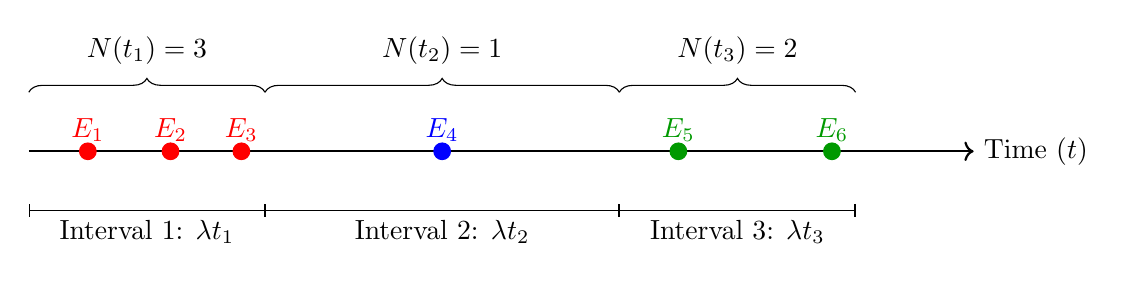
\begin{tikzpicture}[scale=1.5]
    % Timeline
    \draw[->, thick] (0,0) -- (8,0) node[right] {Time ($t$)};
    
    % Intervals
    \draw[|-|] (0,-0.5) -- (2,-0.5) node[midway, below] {Interval 1: $\lambda t_1$};
    \draw[|-|] (2,-0.5) -- (5,-0.5) node[midway, below] {Interval 2: $\lambda t_2$};
    \draw[|-|] (5,-0.5) -- (7,-0.5) node[midway, below] {Interval 3: $\lambda t_3$};
    
    % Events
    \filldraw[red] (0.5,0) circle (2pt) node[above] {$E_1$};
    \filldraw[red] (1.2,0) circle (2pt) node[above] {$E_2$};
    \filldraw[red] (1.8,0) circle (2pt) node[above] {$E_3$};
    
    \filldraw[blue] (3.5,0) circle (2pt) node[above] {$E_4$};
    
    \filldraw[green!60!black] (5.5,0) circle (2pt) node[above] {$E_5$};
    \filldraw[green!60!black] (6.8,0) circle (2pt) node[above] {$E_6$};
    
    % Braces
    \draw [decorate,decoration={brace,amplitude=5pt}] (0,0.5) -- (2,0.5) node [midway,yshift=15pt] {$N(t_1) = 3$};
    \draw [decorate,decoration={brace,amplitude=5pt}] (2,0.5) -- (5,0.5) node [midway,yshift=15pt] {$N(t_2) = 1$};
    \draw [decorate,decoration={brace,amplitude=5pt}] (5,0.5) -- (7,0.5) node [midway,yshift=15pt] {$N(t_3) = 2$};
\end{tikzpicture}
\end{center}
\vspace{1em}

\subsection{Heuristics \& "Cheats"}
\begin{itemize}
    \item \textbf{The "Without Replacement" Trigger:} The moment a problem states "without replacement" from a finite population, immediately write down the Hypergeometric parameters $(N, r, n)$.
    \item \textbf{The "Rate" Trigger:} If a problem gives an average rate (e.g., "3 accidents per month", "5 typos per page"), it is a Poisson distribution. Immediately identify $\lambda$ and ensure the time/space scale matches the question.
\end{itemize}

\subsection{Pitfalls \& Fallacies}
\begin{itemize}
    \item \textbf{Time-Scaling Fallacy:} Forgetting to scale $\lambda$ in a Poisson process. If $\lambda = 2$ per hour, the rate for 3 hours is $\lambda = 6$. Do not use $\lambda = 2$ and multiply the final probability by 3!
    \item \textbf{Binomial vs. Hypergeometric Trap:} Using the Binomial distribution when $N$ is small. If the sample size $n$ is more than $5\%$ of the population $N$, the independence assumption of the Binomial fails, and the Hypergeometric \textit{must} be used.
\end{itemize}

\newpage
\section{Part 5: Conceptual Synthesis and The "Big Picture"}

\subsection{A) Thematic Connections}
The central theme of this chapter is the mathematical formalization of \textit{counting}. We transition from discrete, finite, and dependent counting (Hypergeometric) to infinite, continuous, and independent counting (Poisson). The Binomial distribution acts as the theoretical bridge between the two. By taking the limit as the population size $N \to \infty$, the Hypergeometric converges to the Binomial. By taking the limit as the number of trials $n \to \infty$ while the success probability $p \to 0$, the Binomial converges to the Poisson. This beautifully unifies finite combinatorics with continuous measure theory.

\subsection{B) Forward and Backward Links}
\textbf{Backward Links:} This topic relies heavily on foundational set theory (partitioning sample spaces) and combinatorics (combinations and permutations) learned in introductory discrete math. \\
\textbf{Forward Links:} Understanding the Poisson distribution is the absolute bedrock for advanced Stochastic Calculus. The Poisson process is the fundamental building block for modeling "jumps" in continuous-time Markov Chains, Queuing Theory, and L\'{e}vy processes.

\section{Part 6: Abstract Real-World Modeling (AI, ML, \& Quant Finance)}

\subsection{A) Concrete Scenarios}
\begin{enumerate}
    \item \textbf{High-Frequency Trading (HFT):} The arrival of limit orders in an electronic order book is modeled as a Poisson Point Process. The time between arrivals dictates algorithmic execution strategies.
    \item \textbf{Generative AI \& NLP:} In Large Language Models (LLMs), the occurrence of rare vocabulary words across a massive corpus is modeled using Poisson distributions to optimize tokenization and embedding spaces.
    \item \textbf{Quantitative Finance (Credit Risk):} The default of a corporation on its debt is modeled as a rare event using a Poisson process, forming the basis of Credit Default Swap (CDS) pricing.
\end{enumerate}

\subsection{B) Model Problem Setup: Jump-Diffusion in Asset Pricing}
Standard Black-Scholes models assume asset prices follow Geometric Brownian Motion (continuous paths). However, real markets experience sudden crashes (jumps). We model this using Merton's Jump-Diffusion Model.

Let $(\Omega, \mathcal{F}, \{\mathcal{F}_t\}_{t \ge 0}, \mathbb{P})$ be a filtered probability space. We define the asset price $S_t$ via the Stochastic Differential Equation (SDE):
\[ \frac{dS_t}{S_{t-}} = \mu dt + \sigma dW_t + (J_t - 1) dN_t \]
\textbf{Definitions:}
\begin{itemize}
    \item $W_t$ is a standard Brownian motion adapted to $\mathcal{F}_t$, capturing continuous market volatility.
    \item $N_t \sim \text{Poisson}(\lambda t)$ is a Poisson process counting the number of macroeconomic shocks (jumps) up to time $t$.
    \item $J_t$ is a sequence of i.i.d. log-normal random variables representing the magnitude of the jump.
\end{itemize}
\textbf{Optimization Problem:} To price a European call option under this measure, a quantitative researcher must solve the partial integro-differential equation (PIDE) derived from It\^{o}'s Lemma for jump processes, integrating over the Poisson measure to find the risk-neutral expectation $\mathbb{E}^{\mathbb{Q}}[e^{-rT}\max(S_T - K, 0)]$.

\newpage
\section{Part 7: Common Variations and Untested Concepts}

\subsection{The Negative Hypergeometric Distribution}
While the standard Hypergeometric distribution counts the number of successes in a fixed sample size $n$, the \textbf{Negative Hypergeometric Distribution} models the \textit{waiting time} (number of draws) required to achieve exactly $k$ successes when sampling without replacement.

\begin{theorem}
Let a population of size $N$ contain $r$ successes. Let $X$ be the number of draws required to obtain exactly $k$ successes. The PMF of $X$ is:
\[ P(X = x) = \frac{\binom{x-1}{k-1} \binom{N-x}{r-k}}{\binom{N}{r}} \]
where $k \le x \le N - r + k$.
\end{theorem}

\begin{proof}[Proof of Variation]
To require exactly $x$ draws to get $k$ successes, two independent conditions must be met simultaneously:
1. In the first $x-1$ draws, we must obtain exactly $k-1$ successes.
2. On the $x$-th draw, we must obtain a success.

Alternatively, we can use a combinatorial symmetry argument. Imagine laying out all $N$ items in a row. There are $\binom{N}{r}$ total ways to position the $r$ successes. 
For the $k$-th success to land exactly on the $x$-th position:
- We must choose $k-1$ positions for the earlier successes from the first $x-1$ available spots: $\binom{x-1}{k-1}$ ways.
- We must choose the remaining $r-k$ positions for the later successes from the remaining $N-x$ spots: $\binom{N-x}{r-k}$ ways.
Dividing the product of these choices by the total unrestricted arrangements $\binom{N}{r}$ yields the PMF. $\blacksquare$
\end{proof}

\newpage
\section{Part 8: Advanced Diagnostic Testing: "Find the Flaw"}

Below are five advanced proofs/solutions containing a single, subtle logical or mathematical flaw. 

\subsection{Problem 1: The Limit of Dependence}
\textbf{Problem:} Prove that for a Hypergeometric random variable $Y$, the probability of drawing $y$ successes can be calculated by assuming independent draws if the population $N$ is large. \\
\textbf{Flawed Proof:} As $N \to \infty$, the draws become independent because removing one item does not significantly change the probabilities. Therefore, by the definition of independence, $P(Y=y) = \binom{n}{y} (r/N)^y (1 - r/N)^{n-y}$. $\blacksquare$

\subsection{Problem 2: The Inverse Expectation}
\textbf{Problem:} Let $Y \sim \text{Poisson}(\lambda)$. Calculate $\mathbb{E}[Y^{-1}]$. \\
\textbf{Flawed Proof:} By the Law of the Unconscious Statistician (LOTUS), $\mathbb{E}[Y^{-1}] = \sum_{y=0}^\infty \frac{1}{y} \frac{\lambda^y e^{-\lambda}}{y!}$. We factor out $\lambda$ and shift the index to get $\mathbb{E}[Y^{-1}] = \frac{1}{\lambda} \sum_{y=1}^\infty \frac{\lambda^{y-1} e^{-\lambda}}{(y-1)!} = \frac{1}{\lambda}$. $\blacksquare$

\subsection{Problem 3: The Additive Process}
\textbf{Problem:} A Poisson process has a rate of $\lambda = 2$ arrivals per hour. Find the probability of exactly 2 arrivals in the first hour and 3 arrivals in the second hour. \\
\textbf{Flawed Proof:} The total time is 2 hours, so the rate for the entire period is $\lambda^* = 4$. We want a total of $2 + 3 = 5$ arrivals. Therefore, the probability is $P(Y=5) = \frac{4^5 e^{-4}}{5!}$. $\blacksquare$

\subsection{Problem 4: The Ordered Draw}
\textbf{Problem:} Calculate the probability of drawing 3 red and 2 black cards from a standard deck of 52 cards without replacement. \\
\textbf{Flawed Proof:} The number of ways to draw 3 red cards is $P(26, 3)$ and 2 black cards is $P(26, 2)$. The total ways to draw 5 cards is $P(52, 5)$. So the probability is $\frac{P(26,3) P(26,2)}{P(52,5)}$. $\blacksquare$

\subsection{Problem 5: The Converse of Sums}
\textbf{Problem:} Show that if the sum of two independent random variables $X$ and $Y$ has an expectation of $\lambda_1 + \lambda_2$, then $X+Y$ is Poisson distributed. \\
\textbf{Flawed Proof:} Let $X \sim \text{Poisson}(\lambda_1)$ and $Y \sim \text{Poisson}(\lambda_2)$. By linearity of expectation, $\mathbb{E}[X+Y] = \lambda_1 + \lambda_2$. Since the expectation matches the parameter of a Poisson distribution with rate $\lambda_1 + \lambda_2$, the sum $X+Y$ must follow a Poisson distribution. $\blacksquare$

\vspace{2em}
\hrule
\vspace{2em}

\subsection{Solution Key: Resolutions to the Flaws}

\textbf{Resolution 1:} The flaw is treating a limit as an exact equality. For any finite $N$, the draws are strictly dependent. The equality $P(Y=y) = \binom{n}{y} p^y (1 - p)^{n-y}$ holds \textit{only} in the limit as $N \to \infty$ with $r/N \to p$. It is an approximation, not an exact calculation for finite $N$.

\textbf{Resolution 2:} The flaw is a division by zero. The summation for LOTUS starts at $y=0$. The first term in the sum is $\frac{1}{0} \frac{\lambda^0 e^{-\lambda}}{0!}$, which is mathematically undefined. Therefore, the expectation $\mathbb{E}[Y^{-1}]$ does not exist (it is infinite).

\textbf{Resolution 3:} The flaw is ignoring the specific intersection of events. Calculating $P(Y=5)$ for the 2-hour block includes scenarios like 0 arrivals in the first hour and 5 in the second. By the independent increments property, one must multiply the probabilities of the disjoint intervals: $P(N(1)=2) \times P(N(2)-N(1)=3) = \left(\frac{2^2 e^{-2}}{2!}\right) \left(\frac{2^3 e^{-2}}{3!}\right)$.

\textbf{Resolution 4:} The flaw is a mismatch in ordering. The numerator assumes a specific order (first 3 are red, next 2 are black), while the denominator assumes any order of 5 cards. To fix this using permutations, one must multiply the numerator by $\binom{5}{3}$ to account for all possible interleavings of red and black cards. Alternatively, just use combinations: $\frac{\binom{26}{3}\binom{26}{2}}{\binom{52}{5}}$.

\textbf{Resolution 5:} The flaw is the logical fallacy of Affirming the Consequent. Just because a distribution has a mean of $\lambda_1 + \lambda_2$ does not mean it is a Poisson distribution (e.g., a constant variable $C = \lambda_1 + \lambda_2$ has the same mean). To rigorously prove the sum is Poisson, one must use convolution of PMFs or Moment Generating Functions (MGFs).

\end{document}